\chapter{Modelagem do sistema}  \label{chp:modelagem}
    
    O Pendulo Invertido Dinâmico é um sistema MIMO pois possui duas entradas e três saídas, como pode ser visto na Figura \ref{subsistemas}. Mas se dividido em subsistemas, eles podem ser modelados com técnicas elaboradas para sistemas SISO.
    
    \begin{figure}[h]
        \centering
        \includegraphics[width=15cm]{Imagens/sistemasMIMO.png}
        \caption{Subsistemas da planta de controle}
        \label{subsistemas}
    \end{figure}
        
	\section{Metodologia}
		%\subsection{Caixa cinza}
		Para desenvolver a modelagem dos subsistemas, será adotada a metodologia de desenvolvimento chamada "caixa branca", que consiste em gerar equações diferenciais ordinárias que representem a dinâmica do sistema, a partir de leis físicas básicas. Depois, os parâmetros conhecidos são adicionados a equação final.~\cite{book:dorf}
		
		A lei básica em que a modelagem da equações diferenciais irá partir é a segunda lei de newton, na sua forma linear, dada pela expressão
        
        \begin{equation}
            \sum \vec F  = \frac{d \vec p}{dt},
            \label{SegundaLeiDeNewton}
        \end{equation}
		%
		em que $\sum \vec F$ é a somatória das forças que atuam no corpo e $\vec p$ é o momento linear do corpo.
		
		Ela também será usada na sua forma angular, que se torna
		
		\begin{equation}
            \sum \vec M  = \frac{d \vec L}{dt},
            \label{SegundaLeiDeNewtonRotações}
        \end{equation}
        %
        em que $\sum \vec M$ é a somatória dos momentos de uma força que atuam no corpo e $\vec L$ é o momento angular do corpo.
        
        Depois de modeladas as equações diferenciais, é a plicada a transformada de Laplace para realizar a troca de domínio, do tempo para a frequência, e por fim, é obtida a função de transferência do sistema (resposta ao impulso) dividindo a saída pela entrada.
		
	\section{Modelagem da velocidade tangencial} \label{sec:modelagemvelocidade}
	
	    Faz-se necessário de criar um referencial móvel no espaço, mas fixo na planta, já que, esta se desloca no espaço-tempo. Este referencial terá como nome dos eixos coordenados: $x$, $y$ e $z$, sendo estes perpendiculares entre si, $z$ colinear com o eixo da roda traseira e $y$ normal ao plano que contem o eixo de ambas rodas.
	    
	    \begin{figure}[h]
            \centering
            \includegraphics[width=10cm]{Imagens/MotinhaLateral2.jpg}
            \caption{Vista Lateral da Planta}
            \label{img:velocidade}
        \end{figure}
	    
		A dinâmica da velocidade tangencial, $v$, pode ser modelada considerando que toda massa da planta, $m$, se concentra no seu centro de gravidade, $C_G$, que a planta percorre uma superfície plana perpendicular a gravidade, que existe um atrito equivalente da rolagem das duas rodas, $a$, onde atua uma força externa $F_t$ (oriunda do torque que o atuador traseiro proporciona). Na Figura \ref{img:velocidade} essas variáveis são representadas.
        
        \begin{figure}[h]
            \centering
            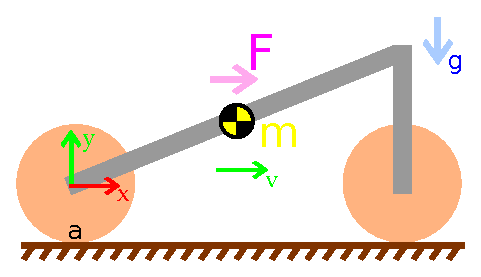
\includegraphics[width=10cm]{Imagens/velocidade.eps}
            \caption{Desenho Lateral da Planta}
            \label{img:velocidade}
        \end{figure}
        
        De acordo com~\cite{book:goldstein} o momento linear de um corpo rígido é dado por
        
        \begin{equation}
            \vec p = m\vec v.
        \end{equation}
        
        Aplicando a segunda lei de newton, na forma escalar para o eixo $x$, temos que
        
        \begin{equation}
            \sum F_x  = \frac{dp}{dt} = m\frac{dv}{dt}.
        \end{equation}
        
        As forças que atuam no sistema são apenas a força de atrito e a força oriunda do torque do atuador, logo
        
        \begin{equation}
            \sum F_x = F_t - av.
        \end{equation}
        
        Igualando as duas equações acima, temos que
        
        \begin{equation}
            m\dot v = F_t - av.
        \end{equation}
        
        A força $F_t$ é oriunda do torque $\tau _t$ que o motor aplica na roda através de uma transmissão por polia-correia, conforme a Figura \ref{img:polia}.
        
        \begin{figure}[h]
            \centering
            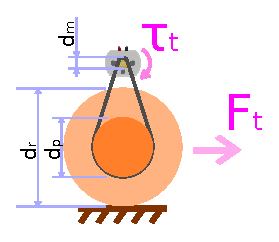
\includegraphics[width=5cm]{Imagens/polia.eps}
            \caption{Desenho da planta - Roda traseira com polia-correia}
            \label{img:polia}
        \end{figure}

        O torque que a roda recebe do motor, $\tau _r$, é dado por
        
        \begin{equation}
            \tau _r = \frac{d_p}{d_m}\tau _t.
        \end{equation}
        
        Logo, a força, $F_t$, oriunda do torque do motor é dada por
        
        \begin{equation}
            F_t
            = \frac{\tau _r}{d_r}
            = \frac{d_p}{d_m d_r}\tau _t .
        \end{equation}
        
        Portanto a equação diferencial se torna
        
        \begin{equation}
            m\dot v = \frac{d_p}{d_m d_r}\tau _t  - av.
        \end{equation}
        
        Como o torque do motor, $\tau_t$, depende da tensão aplicada do motor, $\epsilon_t$, e sua velocidade angular, $\omega_t$, conforme Equação \eqref{eq:torquemotor}, temos que
        
        \begin{equation}
            m\dot v = \frac{d_p}{d_m d_r} (\frac{K_m}{R_a}\epsilon_t - \frac{K_m^2}{R_a}\omega_t) - av,
        \end{equation}
        %
        mas $\omega_t$ é diretamente proporcional a $v$, logo pode ser escrito como
        
        \begin{equation}
            \omega_t = \frac{d_p}{d_m d_r} v,
        \end{equation}
        %
        então a equação diferencial se torna
        
        \begin{equation}
            m\dot v = \frac{d_p}{d_m d_r} (\frac{K_m}{R_a} \epsilon_t - \frac{K_m^2}{R_a}\frac{d_p}{d_m d_r} v) - av,
        \end{equation}
        %
        realizando a distributiva no termo $\frac{d_p}{d_m d_r}$ temos
        
        \begin{equation}
            m\dot v = \frac{d_p}{d_m d_r} \frac{K_m}{R_a} \epsilon_t - \frac{K_m^2}{R_a} \frac{d_p^2}{d_m^2 d_r^2} v - av,
        \end{equation}
        %
        dividindo ambos lados da equação por $m$ temos
        
        \begin{equation}
            \dot v = \frac{1}{m} \frac{d_p}{d_m d_r} \frac{K_m}{R_a} \epsilon_t - \frac{1}{m} \frac{K_m^2}{R_a}\frac{d_p^2}{d_m^2 d_r^2} v - \frac{a}{m}v.
        \end{equation}
        %
        e isolando o termo $v$ temos
        
        \begin{equation}
            \dot v = \frac{1}{m} \frac{d_p}{d_m d_r} \frac{K_m}{R_a} \epsilon_t - ( \frac{1}{m} \frac{K_m^2}{R_a}\frac{d_p^2}{d_m^2 d_r^2} + \frac{a}{m}) v.
        \end{equation}
        
        A fim de simplificar a equação diferencial e a função de transferência, podemos resumir as constantes em duas genéricas, fazendo
        
        \begin{equation}
            c_1 = \frac{1}{m} \frac{d_p}{d_m d_r} \frac{K_m}{R_a}
        \end{equation}
        %
        e
        
		\begin{equation}
            c_2 = \frac{1}{m} \frac{K_m^2}{R_a}\frac{d_p^2}{d_m^2 d_r^2} + \frac{a}{m}
        \end{equation}
        %
        a equação se torna simplesmente
        
        \begin{equation}
            \dot v = c_1 \epsilon_t - c_2 v.
            \label{eq:edovelocidadesimplificada}
        \end{equation}
        
		\subsection{Obtenção da função de transferência}
		
		    As equações 
		    
		    \begin{eqnarray}
                \mathcal{L} [v(t)] = V(s) ;   \nonumber \\
                \mathcal{L} [ \epsilon_t (t)] = E_t (s),
            \end{eqnarray}
            %
            apresentam a relação entre as variáveis no domínio do tempo e no domínio da frequência, após a aplicação da transformada de Laplace.
            
            Aplicando a Transformada de Laplace em ambos lado da E.D.O. \eqref{eq:edovelocidadesimplificada}, temos
            
            \begin{equation}
                V(s) s - v(0) = c_1 E_t - c_2 V(s).
            \end{equation}
            
            A condição inicial será considerada nula, ou seja, $v(0) = 0$, logo
            
            \begin{eqnarray}
                V(s) s + c_2 V(s) = c_1 E_t(s).
            \end{eqnarray}
            
            Então é obtido a função de transferência arbitraria do subsistema de tração
            
            \begin{equation}
                G(s)
                = \frac{V(s)}{E_t(s)}
                = \frac{c_1}{s + c_2}.
            \end{equation}
		
	\section{Modelagem do angulo de esterço} \label{sec:modelagemvangulo}
		
		A dinâmica do ângulo de esterço pode ser modelada considerando um bloco que rotaciona em torno de um eixo paralelo ao eixo $y$, com momento de inercia em torno desse eixo, $J$, com um atrito rotacional no mesmo, $b$, e sob ação de um torque externo $\tau _d$. O ângulo de esterço, $\alpha$, é medido no plano $xz$ do eixo $x$ até a perpendicular do eixo de giração da roda. As constatações feitas podem ser vistas na Figura \ref{img:alpha}.
		
		\begin{figure}[h]
            \centering
            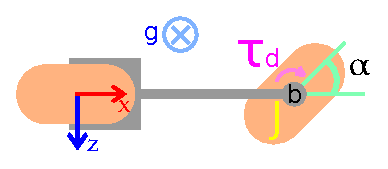
\includegraphics[width=10cm]{Imagens/alpha.eps}
            \caption{Desenho da Planta - Vista Superior}
            \label{img:alpha}
        \end{figure}
        
        De acordo com \cite{book:goldstein}, o momento angular em torno do eixo $y$ é
        
        \begin{equation}
            L_y = I_{xy}\omega_x + I_{yy}\omega_y + I_{yz}\omega_z.
            \label{MomentoAngularOriginal}
        \end{equation}
        
        De acordo também com Goldstain H., quando há dupla simetria no bloco, $I_{xy} = 0 = I_{yz}$, o que é o caso. Já o termo $I_{yy}$ é o momento de inercia do eixo, ou seja, $I_{yy}=J$. Considerando que a velocidade angular em torno do eixo $y$, $\omega_y$, é a derivada temporal do angulo de esterço, ou seja, $\omega_y=\dot \alpha$, temos que
        
        \begin{equation}
            L_y = J \dot \alpha.
        \end{equation}
        
        Aplicando a segunda lei de newton para rotações, Equação \eqref{SegundaLeiDeNewtonRotações}, em sua forma escalar para o eixo $y$, temos que
            
        \begin{equation}
            \sum M_y
            = \frac{d L_y}{dt}
            = J \ddot \alpha.
            \label{eq:segundaleiaplicada}
        \end{equation}
        
        A somatória dos momentos é simples de ser encontrada, apenas dois momentos atuam sobre o pendulo: um é o torque externo provocado pelo motor, e o outro momento é resultado da ação do atrito. Logo
    
        \begin{equation}
            \sum M_y  = \tau _d - b \dot \alpha.
            \label{eq:somatoriamomentosy}
        \end{equation}
    
        Igualando as Equações~\eqref{eq:segundaleiaplicada} e~\eqref{eq:somatoriamomentosy} temos que
        
        \begin{equation}
            J \ddot \alpha  = \tau _d - b \dot \alpha.
        \end{equation}
        
        O dispositivo que atua no angulo de esterço, $\alpha$, é um servo motor, isto é, um motor com redução e com um potenciômetro que mede o angulo do eixo de saída. O momento de inercia equivalente do eixo, $J$, e o atrito equivalente do eixo, $b$, são o resultantes do acoplamento do servo motor com o eixo de direção por intermédio da redução.
        
        O torque, $\tau _d$, que o motor aplica ao eixo depende da tensão aplicada do motor, $\epsilon _d$, e sua velocidade angular, $\omega _d$, conforme Equação \eqref{eq:torquemotor}, considerando $r$ como a razão de redução do servomotor, temos que
        
        \begin{equation}
            J \ddot \alpha = r(\frac{K_m}{R_a}\epsilon_d - \frac{K_m^2}{R_a}\omega_t) - b \dot \alpha,
        \end{equation}
        %
        onde $\omega_m$ é diretamente proporcional a $\dot \alpha$, assim
        
        \begin{equation}
            \omega_m = \dot \alpha r,
        \end{equation}
        %
        então temos que
        
        \begin{equation}
            J \ddot \alpha = \frac{r K_m}{R_a}\epsilon_d - \frac{r^2 K_m^2}{R_a}\dot\alpha - b \dot \alpha,
        \end{equation}
        %
        isolando $\dot \alpha$, temos
        
        \begin{equation}
            J \ddot \alpha = \frac{r K_m}{R_a}\epsilon_d - (\frac{r^2  K_m^2}{R_a} + b) \dot \alpha,
        \end{equation}
        %
        e dividindo ambos lado da equação por $J$, temos
        
        \begin{equation}
            \ddot \alpha = \frac{r K_m}{J R_a}\epsilon_d - (\frac{r^2  K_m^2}{J R_a} + \frac{b}{J}) \dot \alpha.
        \end{equation}
        
        A fim de simplificar tanto a equação diferencial quanto a função de transferência, podemos reunir as constantes das equações em duas contantes $c_3$ e $c_4$. Assim
        
        \begin{equation}
            c3 = \frac{r K_m}{J R_a}
        \end{equation}
        %
        e
        
        \begin{equation}
            c4 = \frac{r^2  K_m^2}{J R_a} + \frac{b}{J},
        \end{equation}
        %
        tornando a equação diferencial
        
        \begin{equation}
            \ddot \alpha = c_3 \epsilon_d - c_4 \dot \alpha.
        \end{equation}
        
        \subsection{Considerações e obtenção da função de transferência}
		
		    A velocidade angular do eixo do motor, $\omega_d$, é diretamente proporcional a derivada temporal do angulo de esterço, $\dot \alpha$. Entretanto tal variável será considerada constante, com valor dado pelo ponto de operação. Dado que a velocidade será regulada pelo controlador em torno do ponto de operação.
		    
		    \begin{eqnarray}
                \mathcal{L} [\alpha(t)] = A(s)   \nonumber \\
                \mathcal{L} [\epsilon_d (t)] = E_d (s)
            \end{eqnarray}
            
            Aplicando a Transformada de Laplace em ambos lado da E.D.O., temos
            
            \begin{equation}
                s^2 A(s) + s\dot\alpha(0) + \alpha(0) = c_3 E_d(s) + c_4 [sA(s) + \alpha(0)].
            \end{equation}
            
            As condições iniciais serão consideradas nulas, ou seja, $v(0) = 0$, logo
            
            \begin{eqnarray}
                s^2 A(s) = c_3 E_d(s) - c_4 A(s)
            \end{eqnarray}
            %
            e então é obtido a função de transferência arbitraria do sistema de ângulo de esterço
            
            \begin{equation}
                H(s)
                = \frac{A(s)}{E_d(s)}
                = \frac{c_3}{s^2 + c_4 s}.
            \end{equation}
		
		
	\section{Modelagem da cinemática da aceleração centrífuga}

        A modelagem do subsistema de inclinação pode ser dividida em duas partes, conforme Figura \ref{subsistemas}, uma responsável por modelar a aceleração centrífuga a partir da velocidade tangencial e angulo de esterço, os dois subsistemas modelados anteriormente, e outro responsável por modelar o angulo de saída $\theta$, a inclinação do pendulo, a partir da aceleração centrífuga. Posteriormente essas duas modelagens podem ser juntadas em uma única equação diferencial que representa a dinâmica do subsistema.

	    Faz-se necessário criar um outro sistema móvel de coordenadas cartesianas, mas agora com a origem no centro de curvatura, o ponto $C$, que é a intersecção dos eixos de giração da roda traseira e dianteira quando a inclinação do pendulo, $\theta$, é $0°$. Esse sistema de coordenadas é chamado $x' y' z'$, onde o eixo $x'$ é paralelo ao eixo $x$, e o eixo $y'$ é perpendicular ao plano do solo, orientado para cima.
	    
	    É necessário nomear a posição do $C_G$ no espaço. Será considerado que posição referente a eixo $z$ é a mesma do centro geométrico da planta. Já para as posições posições referentes ao eixos $x$ e $y$, serão chamadas respectivamente de $d_c$ e $h$. Além disso, a distancia entre eixos será chamada de $d_e$. 
    
        A distância do centro da roda dianteira ao ponto $c$ gera o Raio de Curvatura da Roda Dianteira, $R_d$, a distancia do centro roda traseira ao ponto $C$ gera o Raio de Curvatura da Roda Traseira, $R_t$, e a distancia do $C_G$ ao ponto $C$ gera o Raio de Curvatura do Centro de Gravidade, $R_c$. O ângulo formado entre $R_t$ e $R_d$ é o mesmo ângulo de esterço da roda dianteira, já então $\alpha$. E o ângulo formado entre $R_t$ e $R_c$ é denominado $\beta$. Todas estas esquematizações podem ser vistas na \ref{img:vistasupesquematica}.
        
        \begin{figure}[h]
            \centering
            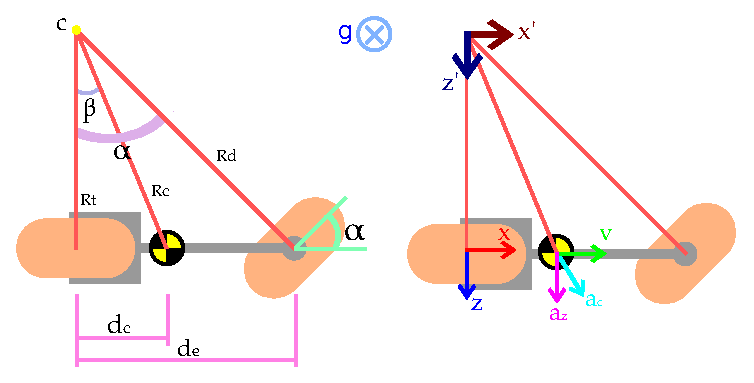
\includegraphics[width=15cm]{Imagens/cinematica.eps}
            \caption{Vista Superior Esquemática da Planta}
            \label{img:vistasupesquematica}
        \end{figure}
        
        A aceleração centrífuga resultante no $C_G$, $a_c$, possui a mesma direção de $R_c$, mas somente a componente $z$ desta aceleração gera momento em $x$, logo, é necessário encontrar a componente $z$ da aceleração $a_c$, ou seja, encontrar $(a_c)_{z}$, que será denominada simplesmente como $a_z$ para tornar as equações mais legíveis. A Figura \ref{img:vistasupesquematica} ilustra essas denominações.
        
	    A planta tem 3 Graus de Liberdade - GLB - medidos, os quais dois deles já foram modelados nas seções anteriores, a velocidade tangencial e o angulo de direção da roda dianteira. O terceiro grau de liberdade, a inclinação do pendulo, depende destas duas variáveis (GLB) citados anteriormente e do tempo.
    
        A forma como essas variáveis influenciam na inclinação do pendulo é gerando uma aceleração centrífuga, que combinada com a gravidade, gera uma aceleração resultante no centro de gravidade que faz o pendulo acelerar rotacionalmente no sentido horário, anti-horário, ou não acelerar. Logo, se faz necessário modelar a aceleração centrífuga em função da velocidade tangencial e do angulo de esterço da roda dianteira. Para encontrar essa relação, e para tal, será feita uma serie de algebrismos trigonométricos.
        
        As variáveis $v$ e $\alpha$ são em funções do tempo, entretanto o parâmetro $(t)$ será omitido a fim de tornar mais elegante as equações, ou seja, $v(t) = v$ e $\alpha(t) = \alpha$.
        
        Primeiro é encontrada a relação entre $R_t$ e $\alpha$.
        
        \begin{equation}
            \tan(\alpha) = \frac{d_e}{R_t} \Rightarrow R_t = \frac{d_e}{\tan(\alpha)}.
        \end{equation}
        
        Através de $R_t$ é possível descobrir $R_c$ sabendo $d_c$,
        
        \begin{eqnarray}
            R_c^2 = R_t^2 + d_c^2 \Rightarrow R_c = \sqrt{R_t^2 + d_c^2} = \sqrt{\frac{d^2}{\tan^2(\alpha)} + d_c^2}.
            \label{eq:rc}
        \end{eqnarray}
        
        É possível obter $\beta$ através das relações já obtidas
        
        \begin{eqnarray}
            \tan(\beta) = \frac{d_c}{R_t} = \frac{d_c \tan(\alpha)}{d}  \Rightarrow \beta = \arctan ( \frac{d_c \tan (\alpha) }{d} ).
            \label{eq:beta}
        \end{eqnarray}
        
        A equação abaixo da a relação entre $a_c$ e $R_c$ sabendo $v$. O ângulo $\beta$ pode ser usado para então encontrar $a_z$
        
        \begin{equation}
            a_c = \frac{v^2}{R_c} \Rightarrow a_z = \frac{v^2}{R_c}cos(\beta).
            \label{eq:az}
        \end{equation}
        
        Substituindo as Equações \eqref{eq:rc} e \eqref{eq:beta} na Equação \eqref{eq:az}, temos que
        
        \begin{equation}
            a_z = \frac{v^2}{\sqrt{\frac{d_e^2}{\tan^2(\alpha)} + d_c^2}}cos(arc\tan(\frac{d_c \tan(\alpha)}{d})).
        \end{equation}
        
        É conhecido que
        
        \begin{equation}
            cos(arc\tan (w)) = \frac{1}{\sqrt{w^2+1}},
        \end{equation}
        %
        logo,
        
        \begin{equation}
            a_z = \frac{v^2}{\sqrt{\frac{d_e^2}{\tan^2(\alpha)} + d_c^2}   \sqrt{(\frac{d_c \tan(\alpha)}{d})^2+1}}.
        \end{equation}
        
        Simplificando e explicitando que $a_z$ é uma função de $\alpha$ e $v$, temos que
        
        \begin{equation}
            a_z(\alpha, v) = \frac{v^2\tan(\alpha)d}{\tan^2(\alpha)d_c^2+d^2}.
        \end{equation}
        
        \subsubsection{Linearizações e simplificações}
    
        A função $a_z(\alpha,v)$ retorna o valor exato da componente $z$ da aceleração centrífuga em função de $\alpha$ e $v$, porém é necessário obter uma função mais simples, através de linearizações e aproximações, para, por exemplo, realizar troca de domínio através da Transformada de Laplace.
        
        Considerando $d_c^2 < d_e^2$, e que $\tan(\alpha)^2 << 1$ para $\alpha$ em torno de $0$, o termo $\tan(\alpha)^2d_c^2$ se torna desprezável em relação a $d_e^2$, ou seja
        
        \begin{equation}
            a_z(\alpha, v) = \frac{v^2\tan(\alpha)d_e}{\tan^2(\alpha)d_c^2+d_e^2} \approx \frac{v^2\tan(\alpha)}{d_e}.
            \label{eq:azdoidão}
        \end{equation}
        
        Linearizando $\tan(\alpha)$ em torno de $\alpha = 0$ utilizando a Serie de Taylor, temos que $\tan(\alpha) \approx \alpha$, logo
        
        \begin{equation}
           a_z(\alpha, v) \approx \frac{v^2\alpha}{d_e} = a_L(\alpha, v).
           \label{eq:LinearizaçãoAlpha}
        \end{equation}
        
        Onde $a_L(\alpha, v)$ também é a aceleração centrífuga decomposta em $z$, em função de $\alpha$ e $v$, entretanto esta função é aproximada e linearizada. A comparação de ambas funções pode ser observada na Figura \ref{img:comparativolinearização}.

		\begin{figure}[H]
            \centering
            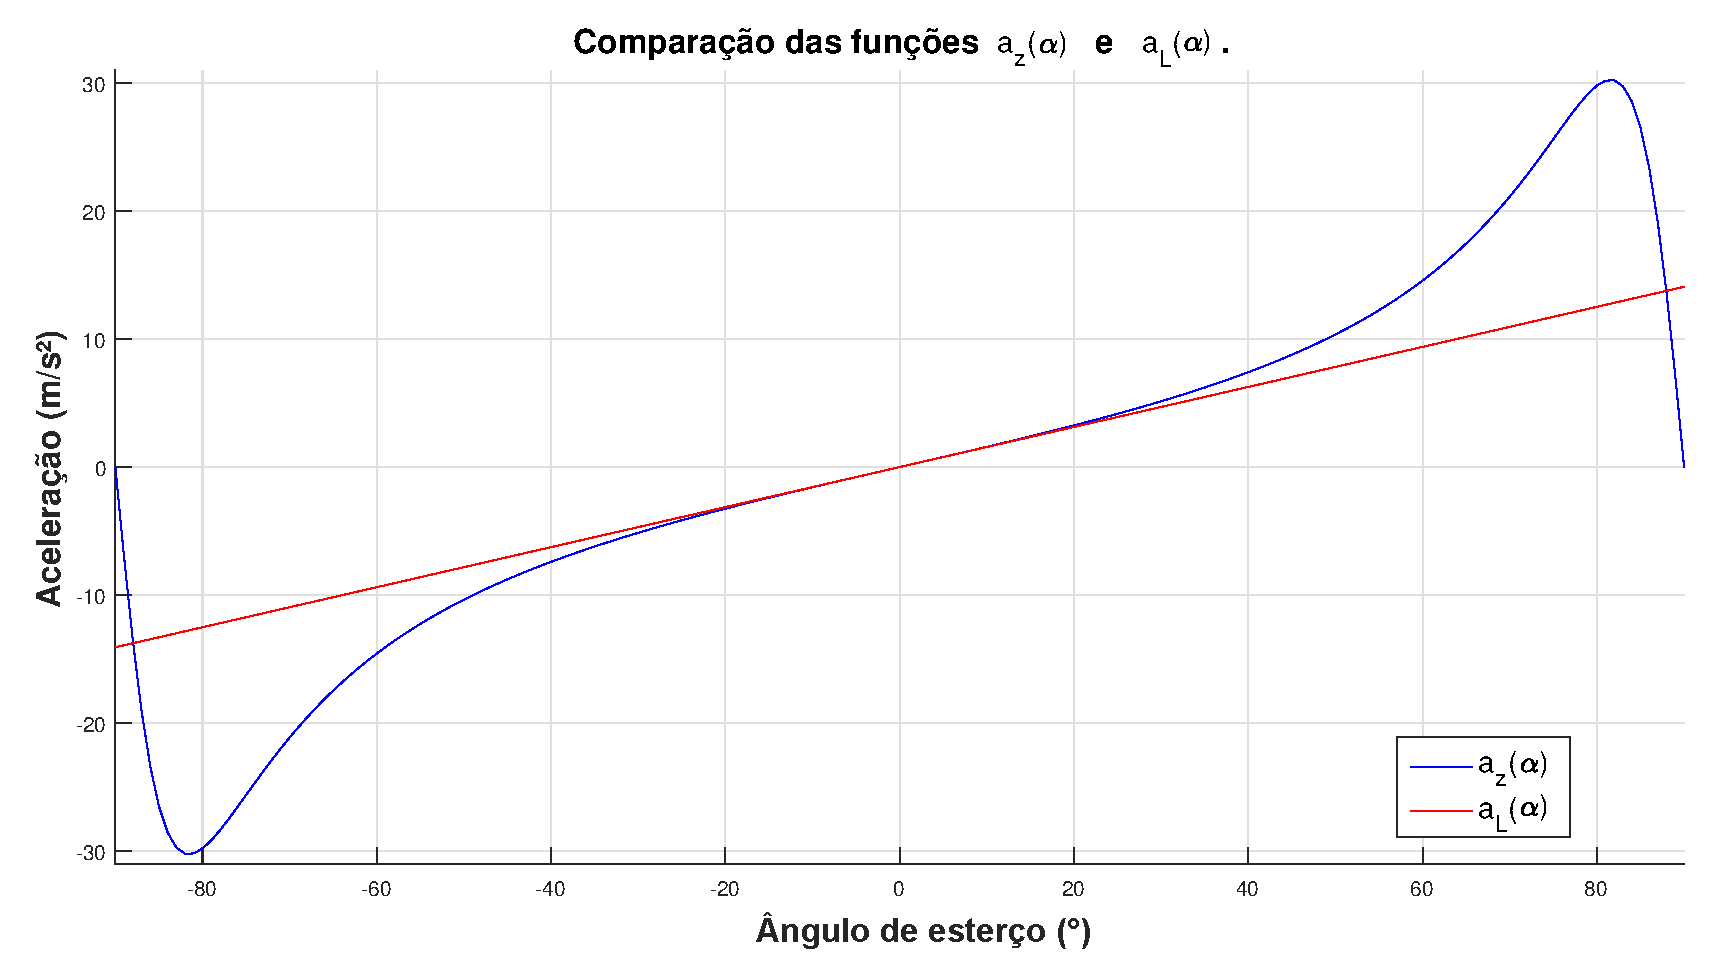
\includegraphics[width=12cm]{Imagens/ComparativoLinearizacao.eps}
            \caption{Comparação entre a função linearizada e não linearizada para um $d_e$ e $d_c$ qualquer.}
            \label{img:comparativolinearização}
        \end{figure}
            
	\section{Modelagem da dinâmica de bicicleta}
        
        Será considerando a planta se movendo por uma superfície plana perpendicular a gravidade, logo, $a_z$ será sempre perpendicular a gravidade, $g$. A aceleração $a_z$ realiza momento em $x$ no $C_G$. O ângulo formado entre a gravidade e o corpo da planta é nomeado de $\theta$, que esta é a variável de saída da planta. A Figura \ref{img:VistaTraseiraEsquematica} ilustra as variáveis citadas.
        
        \begin{figure}[h]
            \centering
            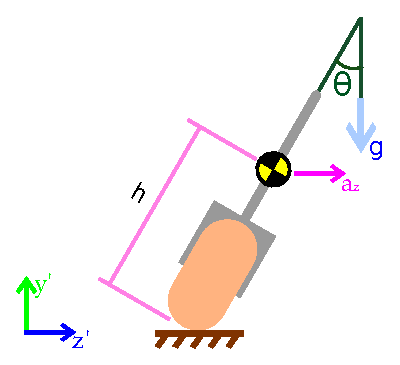
\includegraphics[width=10cm]{Imagens/theta.eps}
            \caption{Vista Traseira Esquemática da Planta}
            \label{img:VistaTraseiraEsquematica}
        \end{figure}
        
        O Pendulo rotaciona em torno do eixo $x$. De acordo com~\cite{book:goldstein}, o momento angular em torno do eixo $x$ é
        
        \begin{equation}
            L_x = I_{xx}\omega_x + I_{xy}\omega_y + I_{xz}\omega_z.
            \label{MomentoAngularOriginal}
        \end{equation}
        
        O termo $I_{xx}$ é o momento de inercia do pendulo em torno do seu eixo de giração. Considerando que toda massa está concentrada em um ponto, o centro de gravidade, temos que:
        
        \begin{equation}
            I_{xx} = mh^2.
        \end{equation}
        
        Já o termo $I_{xz}$ é o produto de inercia para os respectivos eixos $x$ e $z$. Fazendo a mesma consideração do paragrafo anterior, temos que:
        
        \begin{equation}
            I_{xz}=mhd_c.
        \end{equation}
        
        O termo $\omega_x$ é a taxa de variação temporal do angulo $\theta$, descrito na Figura \ref{img:VistaTraseiraEsquematica}. Logo $\omega_x = \dot \theta$.
        
        Como não há rotação em torno do eixo $y$, temos que $\omega_y=0$. Logo não nos interessa saber o valor de $I_{xy}$, pois o produto de ambos será nulo.
        
        E o termo $\omega_z$ é a velocidade angular em torno do ponto $O$. Logo $\omega_z = \frac{v \alpha d_c}{d_e}$.
        
        Substituindo as expressões acima na equação \ref{MomentoAngularOriginal}, temos que
        
        \begin{equation}
            L_x = mh^2 \dot \theta - \frac{vmhd_c}{d_e}\alpha.
        \end{equation}
        
        Aplicando a segunda lei de newton para rotações em sua forma escalar na equação acima, temos que
        
        \begin{equation}
            \sum M_x = \frac{d L_x}{dt} = mh^2 \ddot \theta - \frac{vmhd_c}{d_e}\dot \alpha.
            \label{SegundaLeiDeNewtonRotaçõesAplicada1}
        \end{equation}
        
        A somatória dos momentos é simples de ser encontrada, apenas mois momentos atuam sobre o pendulo: um gerado pela aceleração da gravide, e outro pela aceleração centrífuga, ambos proporcionais a inclinação do pendulo, conforme pode ser visto na Figura \ref{img:VistaTraseiraEsquematica}. Logo
    
        \begin{equation}
            \sum M_x  = a_z(\alpha,v) \cos(\theta)mh + \sin(\theta)mgh,
            \label{SomatorioDosMomentos}
        \end{equation}
        %
        sendo $a_z(\alpha,v) \cos(\theta)mh$ o momento gerado pela aceleração centrífuga e $\sin(\theta)gmh$ o momento gerado pela aceleração da gravidade.
        
        Igualando a equação \ref{SegundaLeiDeNewtonRotaçõesAplicada1} e com a \ref{SomatorioDosMomentos} temos a seguinte equação diferencial
        
        \begin{equation}
            mh^2 \ddot \theta - v\frac{mhd_c}{d_e}\dot \alpha = a_z(\alpha,v) \cos(\theta)mh + \sin(\theta)gmh,
        \end{equation}
        %
        dividindo ambos lados da equação por $mh$, temos

        \begin{equation}
            h \ddot \theta - v\frac{d_c}{d_e}\dot \alpha = a_z(\alpha,v) \cos(\theta) + \sin(\theta)g,
        \end{equation}
        %
        e por fim, substituindo $a_z(\alpha,v)$ pela expressão na Equação \eqref{eq:azdoidão}, temos a equação diferencial não linear
        
        \begin{equation}
            h \ddot \theta - v\frac{d_c}{d_e}\dot \alpha = \frac{v^2\tan(\alpha)d_e}{\tan^2(\alpha)d_c^2+d_e^2} \cos(\theta) + \sin(\theta)g,
        \end{equation}
        
        \subsection{Linearização}
        
            De acordo com \cite{book:dorf}, para obter o modelo em função de transferência, é necessário obter uma Equação Diferencial Ordinária Linear. Primeiramente é preciso definir um ponto de operação. O ponto de operação estabelecido para a entrada e a saída é $(\alpha,\theta)=(0,0)$. Assim sendo, linearizando $sen(\theta)$ e $cos(\theta)$ em torno de $\theta=0$ pela Serie de Taylor obtemos que
            
            \begin{equation}
                cos(\theta) \approx 1
            \end{equation}
            %
            e
            
            \begin{equation}
                sen(\theta) \approx \theta. 
            \end{equation}
            
            Considerando ainda a linearização de $a_z$ dada pela Equação \eqref{eq:LinearizaçãoAlpha} na subseção passada, é possível obter uma equação diferencial linearizada e aproximada para descrever o comportamento da planta
            
            \begin{equation}
                h \ddot \theta -\theta g = \frac{vd_c}{d_e}\dot \alpha +\frac{v^2}{d_e}\alpha,
                \label{eq:edopendulolinear}
            \end{equation}
            %
            em que $\theta$, $\alpha$ e $v$ são funções do tempo, mas o parâmetro $(t)$ foi omitido para tornar as equação mais legíveis.
            
            A dedução dessa equação diferencial, Equação \ref{eq:edopendulolinear}, foi baseada no capítulo Dinâmica de Bicicleta de~\cite{book:astom} e também no artigo~\cite{article:astom}.
            
        \subsection{Considerações e obtenção da função de transferência}
        
            Para modelar o subsistema de inclinação como um sistema SISO, é necessário que ele tenha apenas uma entrada, logo a entrada $v(t)$ será considerada a partir de então como uma constante $v$.
        
            A relação das $\alpha$ e $\theta$ no domínio do tempo com suas respectivas no domínio da frequência é dada por 
            \begin{eqnarray}
                \mathcal{L} [\theta(t)] = \Theta(s)   \nonumber \\
                \mathcal{L} [\alpha(t)] = A(s).
            \end{eqnarray}
            
            Aplicando a Transformada de Laplace em ambos lado da Equação \eqref{eq:edopendulolinear} temos
            
            \begin{equation}
                 \mathcal{L} [h \ddot \theta -\theta g] = \mathcal{L} [\frac{vd_c}{d_e}\dot \alpha +\frac{v^2}{b}\alpha].
            \end{equation}
            
            Como a transformada de Laplace é uma transformada Linear, obtemos o seguinte resultado
            
            \begin{equation}
                h(s^2\Theta(s) - s\theta(t)|_0 - \dot\theta(t)|_0) - g\Theta(s) = \frac{vd_c}{d_e} (sA(s) + \alpha(t)|_0) + \frac{v^2}{b}A(s).
            \end{equation}
            
            As condições iniciais serão consideradas nulas, ou seja, $\alpha(0) = 0$, $\theta(0) = 0$ e $\dot\theta(0)=0$, logo
            
            \begin{eqnarray}
                s^2\Theta(s)h - \Theta(s)g = sA(s)\frac{vd_c}{d_e} + A(s)\frac{v^2}{b}.
            \end{eqnarray}
            
            E então é obtido função de transferência arbitraria do pendulo invertido
            
            \begin{equation}
                Y(s)
                = \frac{\Theta(s)}{A(s)}
                = \frac{\frac{vd_c}{d_e}s + \frac{v^2}{b}} {hs^2 - g}
                = \frac{v}{d_e} \frac{d_cs + v} {hs^2 - g}.
                \label{eq:pendulofinal}
            \end{equation}
                
    \section{Resultados e Discussões}

        A modelagem da função de transferência do pendulo invertido foi feita considerando que velocidade da planta será constante, pois, uma alteração na velocidade altera a dinâmica relacionada, resultando em outra função de transferência, como pôde ser visto na Equação \eqref{eq:pendulofinal}. Por isso, o subsistema de tração será visto como um sistema independente, enquanto os subsistemas de direção e de inclinação é visto como outro sistema. A Figura \ref{img:ModelagemFinal} ilustra melhor o cenário e resume os resultados da modelagem.
        
        \begin{figure}[h]
            \centering
            \includegraphics[width=15cm]{Imagens/sistemasFINAL.png}
            \caption{Sistemas Modelados}
            \label{img:ModelagemFinal}
        \end{figure}
        
        Partindo do pressuposto todos os parâmetros de $G(s)$, $H(s)$ e $Y(s)$ são positivos, o sistema de tração é de primeira ordem assintoticamente estável, pois possui apenas um polo no semi-plano esquerdo do plano $s$. O subsistema de direção é de segunda ordem marginalmente estável, por possuir 2 polos, estando um deles situado na origem do plano $s$, enquanto o outro se localiza no semi-plano esquerdo. E o subsistema de inclinação é instável por possuir um par de polos simétricos no eixo real, ou seja, um dos polos está no semi-plano direito. Além disso, possui um zero cuja posição depende diretamente da velocidade tangencial, $v$ e da distancia em $x$ do centro de gravidade ao eixo roda traseira, $d_c$.
        
        Analisando em termos de projeto de controladores, modelar o sistema dessa forma causa uma limitação ou um desafio de controle. A limitação é que a velocidade tangencial deverá ser constante para o modelo do subsistema de inclinação representar a dinâmica real em torno do ponto de operação. Caso a velocidade sofra alteração, isso gera um desafio de controle, que é o controlador conseguir estabilizar um sistema com variação de parâmetros (a velocidade $v$ no caso, ou seja, a posição do zero).